\renewcommand{\arcsec}{$^{\prime\prime}$} %redundant command definition, but needed for thesis template
\renewcommand{\arcmin}{$^{\prime}$}
\newcommand{\rts}[1]{{\color{violet} RTS: #1}} % RTS comment
\newcommand{\jdp}[1]{{\color{red} JDP: #1}} % JDP comment
\newcommand{\cck}[1]{{\color{brown} CCK: #1}} % CCK comment

\title{First Flight of the EUV Snapshot Imaging Spectrograph (ESIS)}

\begin{abstract}
    This is the abstract.
\end{abstract} 

\section{Introduction}
	\begin{itemize}
        \item Instrument Heritage
            Brief summary since this is a repeat of the instrument paper.
        \item Scientific Motivation and Goals
            There is A LOT of this copied from the proposal into the instrument paper.  I think it needs to be lightly summarized here.
        \item Sections Outline
    \end{itemize}
    

\section{ESIS Mission}
    \begin{itemize}
        \item Brief description of the instrument, mostly pointing to the instrument paper.  Describe ESIS enough so that the data levels make sense. Need to consult the instrument paper to see what fits here. 
        \item ESIS Flight info.  Time, airtime, pointing, stability, etc.  Suggestions welcome here.
        \item Summary of Coordinated Data????
    \end{itemize}
    
	\subsection{The Experiment}
		Description of the instrument/camera, point to the instrument paper
    
	\subsection{Flight Performance} \label{sec:flt}
	
		\begin{center}
			\begin{table}[ht]
				\caption{ESIS Flight Event Timeline (September 30, 2019)}
				\label{tab:timeline}
				\begin{tabular}{lll}\hline
					{\bf} & {\bf Event} & {\bf Time (UTC)}\\ \hline
					0 & Launch        &    ???? \\
					1 & Start Dark Exposures  &  ????\\
					2 & End Dark  Exposures  &  ????\\
					3 & Shutter Door Open     &   ??? \\
					4 & Fine Pointing    &    \\
					& [Ring Laser Gyroscope (RLG) Enable] & ???\\
					5 & Data Acquisition     &     ???\\
					6 & Shutter door close    &   ??? \\ \hline
				\end{tabular}
			\end{table}
		\end{center}
	
		\begin{figure}[ht]
			\begin{center}
				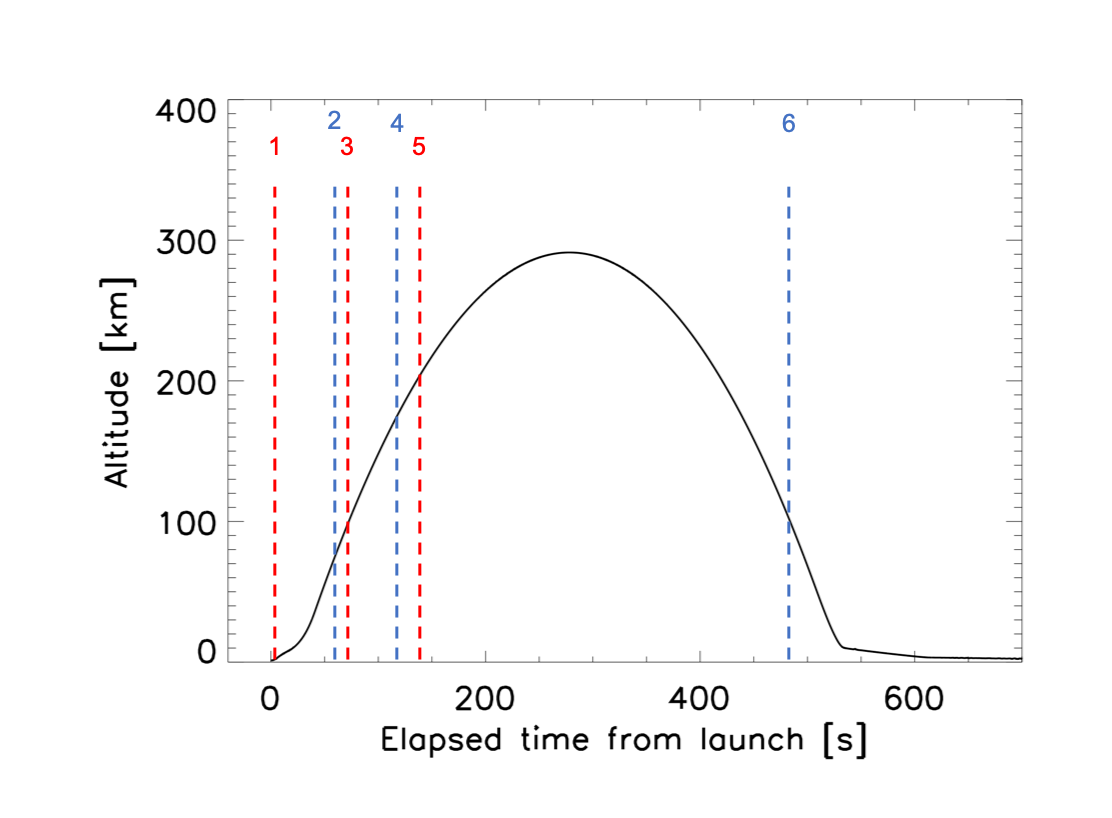
\includegraphics[width=0.7\textwidth]{figures/altevents.png}
				\caption{The altitude of the ESIS rocket determined from White Sands Missile Range radar data as a function of elapsed time from launch.  The event times listed in Table~\ref{tab:timeline} are labeled.}
				\label{fig:timeline}
			\end{center}
		\end{figure}

		ESIS was launched at ????~UT on September 30, 2019 from White Sands Missile Range.  The target of observation was quiet sun at disk center.  The Solar Pointing and Aerobee Control System (SPARCS) maintained a constant target for the duration of the flight.  For ???\,s, ESIS recorded full detector ($\sim$2k$\times$1k) images with a 10\,s exposure and cadence. % Because the time on the Hi-C onboard DACS drifts, an adjustment of 126\,s was applied to all data headers in post-processing. 
		Table~\ref{tab:timeline} provides the timeline of the ESIS rocket flight. Figure~\ref{fig:timeline} provides the height of the sounding rocket as a function of time, determined from White Sands Missile Range radar measurements.  The events given in Table~\ref{tab:timeline} and the approximate height at which they occurred are indicated in this figure.


	\subsection{Pointing} \label{sec:point}
		
		\begin{figure}[ht]
			\begin{center}
%				\includegraphics[width=0.7\textwidth]{}
				\caption{The reference AIA 304\,\AA\ data taken at ???~UT, which was used for determining the absolute pointing. The octagon indicates the ESIS FOV.}
				\label{fig:fov}
			\end{center}
		\end{figure}
	
		\begin{center}
			\begin{table}
				\caption{ESIS Flight Data Summary (*Solar coordinates; solar north at top of frame.)}
				\label{tab:data_info}
				\begin{tabular}{ll | l l}\hline
					Wavelength Range &   ???\,\AA\  & Image Size  & 2064$\times$1024\\
					Launch Date & September 30, 2019 & Field of View  & ?\arcmin octagonal \\
					Data Acquisition Time & ??? - ??? & Pointing  & (-?\arcsec, ?\arcsec)$\pm .3$\arcsec  \\
					Camera Gain &   [4 cameras]$2.5 \pm 0.02$\,elec DN$^{-1}$ & Roll & $??? \pm ???^\circ$ CW \\
					Camera Noise*: & & Exposure Time & 10\,s\\
					\hspace{0.2in}NE Quad & [?,?,?,?] DN & Light Data Set: &\\
					\hspace{0.2in}NW Quad & [?,?,?,?] DN & \hspace{0.2in}No. of Images & 29\\
					\hspace{0.2in}SE Quad  & [?,?,?,?] DN & &\\
					\hspace{0.2in}SW Quad  & [?,?,?,?] DN & Dark Data Set & \\
					Plate Scale  & 0.??\arcsec\ pixel$^{-1}$ &  \hspace{0.2in}No. of Images & ? \\
					\hline
				\end{tabular}
			\end{table}
		\end{center}
		

		To determine the roll offset and absolute pointing post flight, the AIA\,304\,\AA\ image taken at ???~UT was used as a reference against the ESIS images taken at ???~UT.  The roll offset, found to be $\sim0.???\pm 0.005^\circ$ (clockwise about Sun center), is within the tolerances for SPARCS pointing.  Figure \ref{fig:fov} shows the full-disk AIA\,304\,\AA\ image. The ESIS FOV is indicated by the octagon.  
	
\section{Data} 

    ESIS gathers an image in each of its four detectors (channels) during every exposure.  
    Each channel has its own grating and detector and is located around the m = 1 circle in 45 degree increments. (\textbf{also a poor way to say this}
    \cck{Each channel is identical, with its own grating and detector. They are arrayed at $45^{\circ}$ increments about the axis of symmetry of the paraboloidal primary mirror. ESIS has 4 channels currently, but is built to accommodate up to 6 (limited by interference with the optical bench).\footnote{\cck{This all might belong in the instrument description.}}}
    
    \begin{figure}[ht]
        \centering
%       	\includegraphics{}
        \caption{Raw CCD Data}
        \label{fig:Level0}
    \end{figure}
    
    \cck{Refer to raw CCD data as Level 0?}
    We have broken our data prep/analysis pipeline into multiple levels, labeled one through four.
    Level 1 data prepares raw CCD data for scientific work through a quadrant dependent bias subtraction and gain correction, as well as dark subtraction and despiking (optional).
    Level 2 data adds additional metadata \cck{(metadata is all one word)} to the Level 1 data, including a non-linear and wavelength dependent mapping from detector to field stop for use in inversions (work in progress) \rts{This actually kinda works right now} \jdp{ Maybe we'll have an ``in preparation'' to cite for this.}. \cck{Level 2 data is a necessary step toward L4, but will not be further described here. Instead, we seek a shortcut to interpretation of the bright O\,\textsc{v} spectral line, including image differences and simplified inversions.}
    Level 3 data takes a cropped single wavelength from Level 1 data and maps to the sky plane via a non-linear, but wavelength independent mapping. \cck{Nonlinear coordinate transformation (don't want our reader to think it is nonlinear in intensity).}
    And lastly Level 4, represents an inverted \cck{data product in the form of an} $[x, y , \lambda]$ \cck{(Keep all math symbols within \$ ... \$)} cube (\textbf{probably a better way to write this}), the end goal of the ESIS instrument. \cck{The highest level data product we envision, Level 4, is an $[x, y , \lambda]$ data cube, which is the result of an inversion. Since inversion is not unique, there may be multiple L4 products obtained by different methods.}
    Below each complete data level is explored in more detail.
    
    \subsection{Level 1 Data}
    \jdp{Moving Amy's comment about atmospheric absorption to this section.  Roy already has some nice plots of this and it can likely be discussed in a section explaining dark selection?}
    
  
    
    % 	[Copied from Hi-C paper as a reminder that we need to talk about atmospheric absorption somewhere.] We use the normalized total intensities of the Level~1.0 processed flight data (processing levels described in Section~\ref{sec:data}) to assess the relative atmospheric absorption of the signal as a function of flight time.  The transmission, shown in Figure~\ref{fig:absorb} in combination with the payload altitude, is calculated as the inverse of the relative absorption (i.e., (absorption coefficient)$^{-1}$). More than 4 minutes of data were unaffected by the atmosphere.  The atmospheric absorption was compensated for in the Level~1.5 processed data set by multiplying the images by their respective absorption coefficient.  These coefficients are provided in the header of this processed set.
    	
    	
    	A summary of the flight data parameters, as described in the preceding sections, is provided below in Table~\ref{tab:data_info}. 
    	
        The goal is to get a signal proportional to the number of photoelectons. 
        The result of the Level-1 process is the number of photoelectrons 
        The Level-1 dataset is a sequence of images derived from the Level-0 (raw) dataset.
        The images in this dataset have had camera-level effects such as pedestal, gain, and dark current removed.
        Also, the images in this dataset have had the 
        Camera-level effects such as pedestal, gain, dark current, and light-insensitive pixels have been removed from the images in this dataset.
        The images 
        This dataset removes camera-level effects from the Level-0 dataset such as pedestal, gain, dark current and light-insensitive pixels (such as overscan pixels).
        
        
        Also, Level-1 images have the light-insensitive pixels (such as the overscan pixels) removed 
    
        The goals of the Level-1 dataset are to remove camera-level effects (pedestal, gain, and dark current), trim light insensitive pixels, and to remove spikes. to prepare for the images for coalignment.
    
       Raw ESIS data (Figure \ref{fig:Level0}) must first be corrected for quadrant dependant gain and bias, have overscan and blank pixels removed, and be dark subtracted prior to further analysis.
       
	       \cck{Seems like you have tried to write this a few different ways. Maybe starting with a sentence about the goal (signal proportional to photoelectrons), and then presenting an enumerated list of steps. Subsequent narrative can explain any procedures that aren't obvious or straightforward.}


    \subsection{Level 3 Data}
 
    
    	\newcommand{\vigfit}{[0.44, 0.34, 0.38, 0.5]}
    	\newcommand{\levthreetime}{2019-09-30T18:08:51.644}
    	
    	
    	The ESIS Level-3 data product was created to provide a co-aligned, single wavelength image in each channel for quicker identification of events with non-zero LOS velocities, and easier comparison with coordinated data that doesn't require inversion. 
    	It will also allow for single wavelength inversion prior to the completion of a more complete optical distortion model and the Level-2 data product.
    	Figure \ref{fig:coalign}a shows a final Level-3 image from Camera 1 taken at \levthreetime.
    	
  		\begin{figure}[htb!]
    		\centering
    		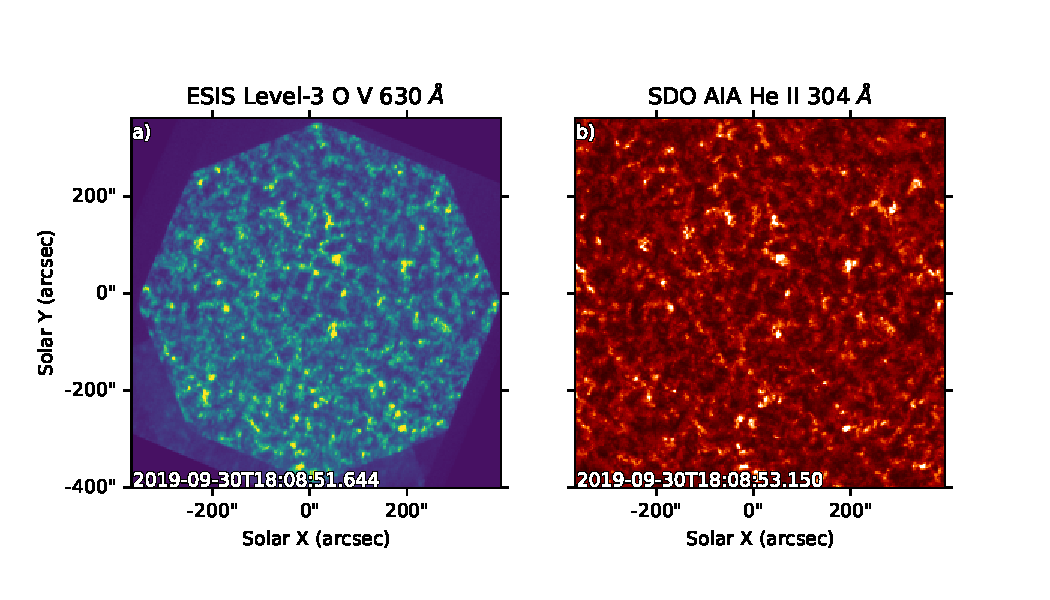
\includegraphics{aia_coalign.pdf}
    		\caption{Caption}
    		\label{fig:coalign}
    	\end{figure}
    	
    
     	In order to use Level-3 data for early inversion the intensity in DN needs to  converted to photons in order properly account for uncertainty and then normalized between channels.
   		Since each ESIS CCD has a quadrant specific gain \citep{ESIS}, the conversion from DN to photon is done to Level 1 data prior to co-alignment efforts.
   		The intensity in photons for each quadrant, $I_q$, then becomes,
   		\begin{equation}
	   		I_q = I_{DN} * Gain_q * 3.6\ \frac{eV}{e^{-}} * \frac{\lambda}{hc}.
   		\end{equation}
   		With an average quadrant gain, $Gain_q$, of $2.56\ electron\ eV^{-1}$, a Silicon band gap energy of $3.6\ eV\ electron^{-1}$, and $19.6\ eV\ photon^{-1}$ each count in $DN \approxeq 0.46$ photons in O V 627.8 \AA .
   		Creating Level-3 data for other wavelengths in the ESIS passband then only requires a different wavelength for conversion.
   		Normalizing the intensity of each channel is done by equalizing the image mean over a shared piece of sun, and is therefore performed after inter-channel co-alignment.
   		
   		The four ESIS channels were spatially co-aligned in two steps.  
   		First, each ESIS image is roughly cropped around the desired spectral line and then co-aligned to the closest AIA 304\,\AA\ image in time.
   		This rough cropping is why there is a remnant of the adjacent Mg {\sc x} 609.8 \AA \ spectral line in the bottom left corner of Figure \ref{fig:coalign}a.
   		AIA 304 was chosen because it is the AIA EUV channel most visually similar to O V, in both the background and bright events (Figure \ref{fig:coalign}b).
   		Prior to co-alignment each AIA image was prepped to Level-1.5 using the aiapy routines \texttt{update\_pointing.py} and \texttt{register.py} \citep{aiapy}.
   		The co-alignment was achieved through a linear transformation of the cropped ESIS image that maximizes the zero lag cross-correlation between it and AIA 304, the results of are shown in Figure \ref{fig:coalign}b.
   		Despite each image being in a different wavelength and at slightly different times we found an average zero lag cross-correlation of approximately $0.45$.
   		After the transformation each ESIS channel is re-binned to AIA resolution and can be assigned the WCS information from AIA Level 1.5 providing pointing information and easier co-alignment with other instruments.

    	Since ESIS has a slightly non-linear distortion function \citep{ESIS}, an additional internal alignment step is performed.
    	Using a single ESIS channel as reference, in this case Camera 2, each other camera is co-aligned to it via a quadratic transformation that maximizes the zero-lag cross-correlation. 
    	After performing this additional internal alignment we find that not only is the zero-lag cross-correlation between each channel and the reference channel improved (dots in Figure \ref{fig:cc}), but also the cross correlation between every other combination of channels (stars in Figure \ref{fig:cc}).
    	Examining the cross-correlation ratio of each camera pair shows a less than 1 percent improvement in peak correlation Figure \ref{fig:cc}, demonstrating the subtle non-linearity of the ESIS optical distortion function.
    	In pixels, this corresponds to an average change in mapping of \jdp{\textbf{FIND THIS}}.
    	
    	\begin{figure}[htb!]
    		\centering
    		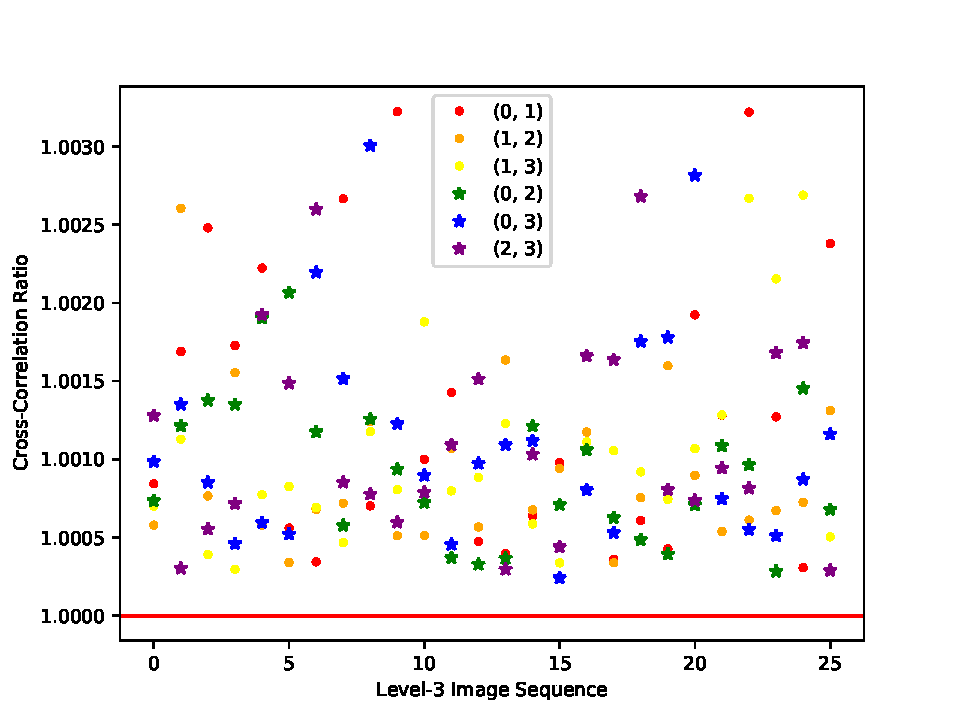
\includegraphics{internal_align.pdf}
    		\caption{For each ESIS exposure (or image sequence) every channel pair, labeled in the legend, is cross-correlated to measure internal alignment quality.  The ratio of zero lag cross-correlation after a quadratic transformation to that of a linear transformation is plotted.  Every point being above the ratio = 1 line indicates improved internal alignment for every combination of ESIS channels for each image sequence.}
    		\label{fig:cc}	
    	\end{figure}
    	
 		\begin{figure}[htb!]
			\centering
			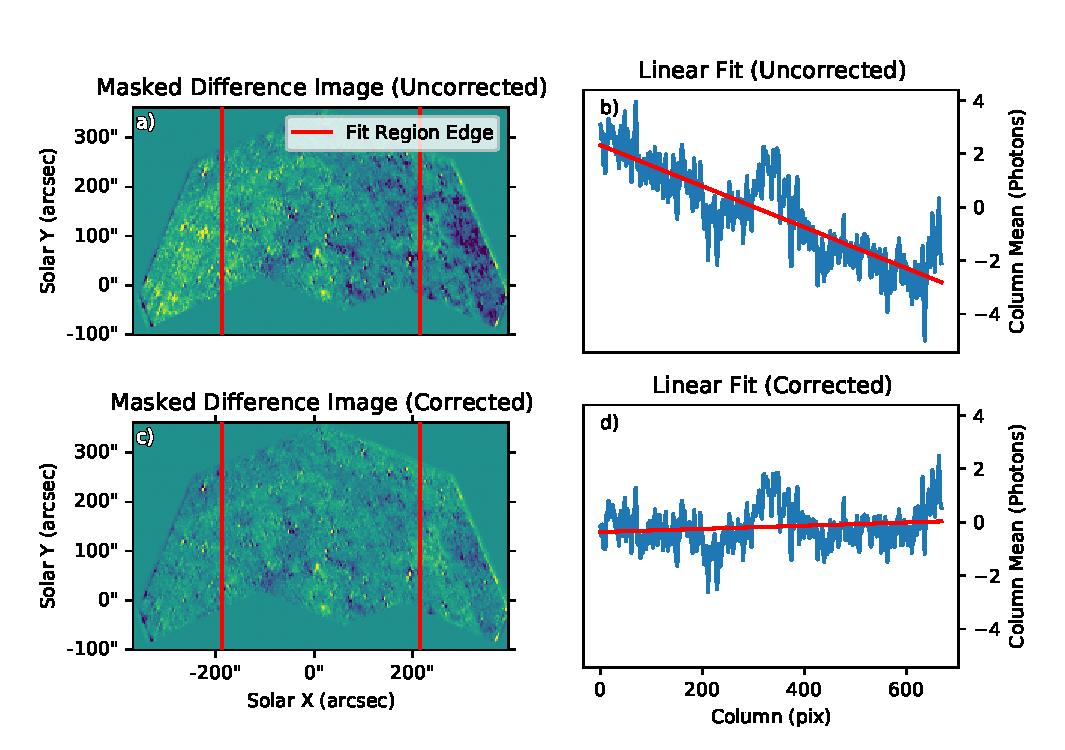
\includegraphics{vig_correct.pdf}
			\caption{Caption}
			\label{fig:vig_correct}
		\end{figure}
	       	
        Each ESIS channel has a linear trend in intensity along the dispersion direction due to internal vignetting in the optical system \citep{ESIS}.
        This linear trend in the background is very apparent in difference images that haven't been corrected (upper left of Figure \ref{fig:vig_correct}).
        To correct the trend, we divide out a linear trending background from each image with a slope oriented to the dispersion direction in each channel.
        The vignetting field divided out for each channel is,
        \begin{equation}
            V_{is} = m_{i} * (r - r_0) + 1,
            \label{eqn:vignet}
        \end{equation}
       	where,
       	\begin{equation}
        	r = x_0 + [cos(\alpha_i)(x-x_0-x_{drift}*s) - sin(\alpha_i)(y-y_0-y_{drift}*s)].
        	\label{eqn:vignet2}
       	\end{equation}
       	In Equation \ref{eqn:vignet}, $r_0$ is equal to 65 pixels, and represents the distance from the Level-3 image edge to the ESIS field stop octagon edge at $s = 0$, the first Level-3 image sequence.
       	Also, $m_{i}$ is the slope of the vignetting field, for each channel $i$, and is a free parameter of the fit.
        In Equation \ref{eqn:vignet2},  $\alpha_i$ is the angle of rotation of each ESIS Level-3 image relative to a Level-1 image row.
        In this case, $\alpha_i = [112.5^{\circ}, 67.5^{\circ}, 22.5^{\circ}, -22.5^{\circ}]$, for cameras one through four respectively.
        The vignetting field is rotated about the origin of each image in pixels, $[x_0, y_0] = [635,635]$, to account for the change in dispersion direction.
        Because ESIS images have a pointing drift as a function of time, or image sequence $s$, the image origin is translated by $[x_{drift},y_{drift}]*s/s_t = [8_{pix},-4_{pix}]*s/26$, where $s_t $ is the total number, 28, of Level-3 images in time.
        
        When fitting for the vignetting field slope, $m_i$, for each  of the four ESIS channels we mask off the portion common to them all with no contribution from Mg {\sc x} 609.8 \AA. \cck{'twould help to have a figure illustrating the overlap of spectral lines. Maybe something already being prepared for another purpose?}
        The four channels of ESIS give 6 possible difference images for fitting the vignetting function for each image sequence $s$. 
        For each difference image we take a mean of each column and fit a line to it as a function of column position, shown in the right hand column of Figure \ref{fig:vig_correct}.
        When the average slope of all 156 fits (6 difference images per each of the 26 exposures) is minimized we consider the vignetting corrected. 
        The resulting final fit, $m_i = \vigfit$, predicts smaller slopes than are predicted using ray tracing and geometric optical models \citep{ESIS}, which can be attributed to a few likely culprits.
        One source of error likely comes from the imprint of adjacent spectral lines, the most obvious being that of Mg {\sc x} 626 \AA \ visible in Figure \ref{fig:vig_correct}c.
        Since this Mg {\sc x} line overlaps almost entirely with O {\sc v}, and has an identical vignetting function, it adds intensity that prevents a perfect fit. \cck{If this were the only source of discrepancy between the vignetting function predicted by the raytrace and the fits obtained from the data, then we would simply use the same, predicted vignetting for every channel. However, we can anticipate slightly different vignetting in each channel due to variations in assembly....}
        Another source of error comes from the ESIS optical system.
        Each channel having a different slope was added as an additional three free parameters, despite the fact that our models predict an identical slope for each channel, because of known possible errors in the build up of ESIS.
        A misalignment of the ESIS field stop center, the ESIS primary optic center, and the center of the ESIS grating array, all shift the geometry of the ESIS central obscuration and can easily modify the vignetting field in each channel.
        Future implementations of a wavelength dependent optical distortion model and the creation of the Level-2 data product will yield a more consistent and contaminant free fit to the vignetting function. \cck{(I don't think it is helpful to make vague promises of a better vignetting estimate in the future, unless perhaps it is tied to global inversions.)}
        Despite these errors \cck{Despite the uncertainties in vignetting, which we have found difficult to quantify}, Level-3 differences are much flatter in intensity post correction as is seen in Figure \ref{fig:vig_correct}c, and will therefore lead to a higher fidelity intensity recovery when inverting Level-3 data.
        

  

\section{Preliminary Results}
	September 30th, 2019 was a very quiet day on the sun.  
	In fact, the last day prior to the ESIS launch that produced a B-class event \citep{GOES} \jdp{figure out how to cite GOES, also, I couldn't believe I had to go back so far so check me on this.}, was July 7th 2019.  
	Because of this exceptionally quiet period on the sun we chose to point at disk center, in order to minimize projection effects.  
	Despite the lack of solar activity ESIS managed to capture one hundred plus small, transient events and one significant eruption during the 5 minutes of observation \jdp{insert actual flight time}.
	
	Early work with MOSES images, very similar to ESIS images, has demonstrated the utility of using differences between channels to identify solar features with significant line-of-sight velocity \citep{???}, and extra spectral content \citep{???}.  
	It is for this reason that we have chosen to develop a data product quickly (Level-3) that would allow us to take differences.  
	Also, simple events viewed in Level-3 difference images are easily interpretable with a little insight into how the instrument works and therefore serve as a sanity check for more complicated inversions. 
	
	In the following subsections we will show a handful of events easily identifiable in the ESIS difference images and explain how their presentation can be interpreted as a red/blue shift or line broadening.  
	We will then demonstrate how simple inversions can be qualitatively validated by these interpretations and show progress toward inverting and interpreting the larger eruption captured by ESIS.
	
    \subsection{Level-3 Difference Images}


      
    	Each ESIS channel disperses features with a non-zero LOS velocity a different direction, determined by the azimuthal position of each grating.
    	The dispersion direction in each Level-3 image can be found by looking for intensity from the nearby Mg {\sc x} 609.8 \AA \ spectral line.
    	In Figure \ref{fig:coalign}a, showing camera 2, this can be seen in the bottom left hand corner.  
   		Since the the Mg {\sc x} line is shorter in wavelength, a blue shifted feature (with velocity toward the observer) would be smeared down and to the left, and a red shifted feature up and to the right.	
   		Stationary solar features present the same in each ESIS channel.
   		Therefore, taking the difference of two channels reveals a variety of interesting features.
   		
   		\begin{figure*}[htb!]
   			\centering
   			% 		\includegraphics{}
   			\caption{Full FOV Difference Image}
   			\label{fig:l3_dif}
   		\end{figure*}

    	Features in an ESIS difference image that have obvious and nearby positive and negative portions indicate solar events with significant LOS Doppler velocity.
    	Simple, point like, transient brightenings with little to no spatial structure are the most easily interpretable of these features.
    	\jdp{very well described in \citet{Rust2019} Section 1.3.1 I think.  Try to incorporate this.} 
    	Taking the difference of these small events leaves a V-shaped or X-shaped structure in it's place.
    	In these simple events, a qualitative understanding of their velocity can be ``read off'' of the difference images.
    	For example, Figure \ref{fig:dif_events}a shows a V-shaped event that is pointed upward in the difference between the Camera 2 and Camera 3 Level-3 image.
    	Since we know that the direction of positive wavelength dispersion is up and to the right in Camera 2 and up and to the left in Camera 3 we immediately know that this event is predominantly red shifted.
    	For opposite reasons, a downward facing V-shaped event, Figure \ref{fig:dif_events}b, is predominantly blue shifted.
    	Therefore, X-shaped events (Figure \ref{fig:dif_events}c), that occur equally if not more frequently than V-shaped events, indicate significant line broadening.
    	While this gives us a quick and qualitative understanding of an event, even the smallest amount of spatial extent in a given feature leads to an entanglement of spatial and spectral information makes it very difficult to derive qualitative velocities without inversion. 
    	
    	\begin{figure}[htb!]
    		\centering
    		\caption{An example of a red, blue, and broadened transient brightenings.}
    		\label{fig:dif_events}
    	\end{figure}
    	
    	While ESIS images are littered with these simple ``point-like'' events, we also captured a handful spatially extended that are more difficult to interpret.
    	The most obvious of these is a much larger eruption just below disk center \jdp{get some arcsecs}
    	In difference images of this event we see a mess of positive and negative features intertwined in the brightest section that sometimes present as a V or X shape, but not always, and change their presentation significantly over time.
    	There is also and imprint of fainter differences above the brightest knot of intensity showing motion along a spatially extended structure, likely from material being ejected from the eruption site.
    	Dynamic and spatially extended events are excellent opportunities for ESIS to shine and clearly demonstrate the need for many different projection angles (ESIS channels) if we hope to disentangle spatial information from spectra.
    	Despite the extra complexity, out understanding of ESIS difference images provides an excellent sanity check when interpreting future inversions.
    	
    	Larger positive or negative features with no obvious counterpart nearby, are indicative of extra spectral content \citep{RustThesis,MCOR}.
    	The most easily seen impact of this is a faint octagon edge visible in Figure \ref{fig:l3_dif} from Mg {\sc x} 625.9 \AA.
    	Extra spectral content will act as a source of error when inverting Level-3 data, but will be properly accounted for by a wavelength dependent optical distortion model and the completion of the ESIS Level-2 data set \citep{Smart2022}. 	
    
    \subsection{Early Inversions}
    	In order to better disentangle the spectral and spatial information captured by ESIS, information from every channel is combined and "inverted" to return a single, spatial-spectral cube, at every exposure.
    	In general, each method of inversion starts with a spatial-spectral cube, passes it through a forward model of the ESIS optical system generating an image per channel, then compares each synthetic image to actual ESIS data.
    	For out preliminary inversions of Level-3 data we use a Smoothed Multiplicative Algebraic Reconstruction Technique (SMART) used previously on MOSES data \citep{}, but with a new forward model of the ESIS instrument.
    	MART (Multiplicative Algebraic Reconstruction Technique)
    	
    	
\section{Discussion/Conclusions and Future Work}

